\documentclass{article}
\usepackage[english]{babel}
\usepackage[letterpaper,top=2cm,bottom=2cm,left=3cm,right=3cm,marginparwidth=1.75cm]{geometry}
\usepackage{amsmath}
\usepackage{graphicx}
\usepackage{algorithmicx}
\usepackage{algorithm}
\usepackage[colorlinks=true, allcolors=blue]{hyperref}

\title{\textbf{CS456: Algorithm Design and Analysis}}
\author{Elikem Asudo Tsatsu Gale-Zoyiku}
\date{9th Februrary, 2024}

\begin{document}
\maketitle
\begin{center}
    \begin{large}
        \textbf{Assignment 2\\}
    \end{large}
\end{center}
\newpage
\section*{Question 1}
\begin{enumerate}
    \item Constant Factor in Execution Time:
          The data shows that the count, representing the algorithm's execution time, consistently falls within a narrow range (between 11 and 13 times the input size) across various input sizes.
          \begin{itemize}
              \item For instance, with an input size of 2000, the count is 24,303, and with an input size of 3000, the count is approximately 39,992.
              \item Calculating the ratio of count to input size for each data point reveals a nearly constant factor, around 12, regardless of the input size.
              \item Consider the data point with an input size of 1000: Count is approximately 11,966.
                    Calculating the ratio of count to input size: \( \frac{11966}{1000} \approx 11.966 \).
                    Similarly, for the data point with an input size of 2000: Count is approximately 24,303, and the ratio is \( \frac{24303}{2000} \approx 12.152 \).
                    Despite doubling the input size from 1000 to 2000, the ratio remains close to 12, indicating a nearly constant factor.
          \end{itemize}

    \item Linear Relationship:
          \begin{itemize}
              \item Doubling the input size approximately doubles the count, demonstrating a linear relationship between the input size and the count. For example, when the input size increases from 1000 to 2000, the count roughly doubles from 11,966 to 24,303.
              \item Take the example of doubling the input size from 2000 to 4000.
                    With an input size of 2000, the count is around 24,303, and with an input size of 3000, the count is approximately 53,010.
                    The ratio of counts is \( \frac{53010}{24303} \approx 2 \).
                    Doubling the input size approximately doubles the count, demonstrating a linear relationship.
                    This consistent doubling behavior across different input sizes indicates that the execution time scales linearly with the size of the input data.
          \end{itemize}
          These two observations suggest that the algorithm's execution time has a linear relationship with the input size, with a nearly constant factor. This implies that the algorithm has a time complexity of \( O(n) \), where \( n \) is the input size.

    \item Graphical Representation:

          To visually illustrate these observations, the data points have been plotted on a graph with the input size on the x-axis and the count on the y-axis.
          The graph clearly depicts a linear relationship, where the data points form a straight line with a positive slope.
          This linear behavior on the graph further reinforces the hypothesis of linear time complexity (O(n)) for the algorithm, as it demonstrates that the execution time increases linearly with the input size.
          The graph can be seen below:
          \begin{center}
              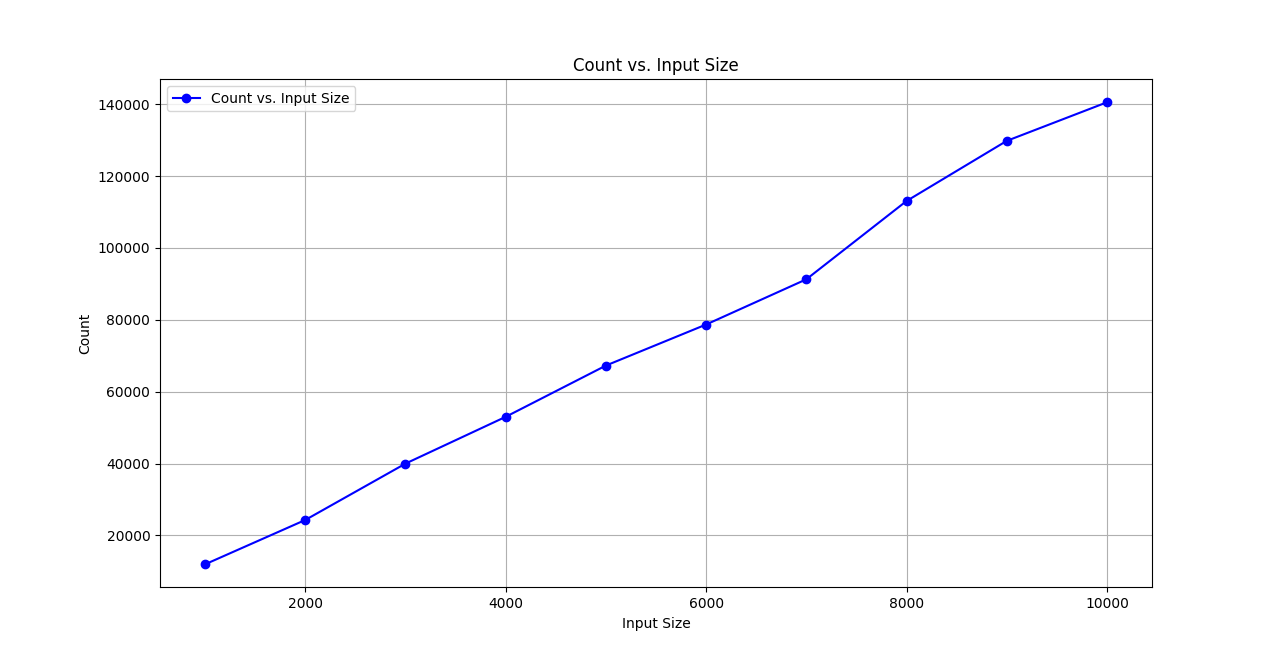
\includegraphics[width=0.9\textwidth]{graph.png}
          \end{center}
\end{enumerate}
\newpage
\section*{Question 2}
\subsection*{a}This algorithm computes the minimum value in an array of real numbers.
It recursively searches for the minimum value by comparing elements of the array.
The base case is when the array contains only one element, in which case the algorithm returns that element as the minimum value.
Otherwise, it recursively finds the minimum value in the subarray A[0 .. n-2] and compares it with the last element of the array (A[n-1]).
If the minimum value from the subarray is less than or equal to the last element, it returns the minimum value from the subarray.
Otherwise, it returns the last element of the array as the minimum value.

\subsection*{b}
Let the basic operation count of the algorithm as T(n), where n is the size of the input array A.

The basic operations in this algorithm are comparisons and recursive calls.
\begin{itemize}
    \item Comparisons: There are (n-1) comparisons made in the worst case scenario when checking each element of the array to find the minimum value.
    \item Recursive Calls: The algorithm makes one recursive call for each element of the array except for the first one. Therefore, there are (n-1) recursive calls in total.
\end{itemize}
Hence, the recurrence relation for the algorithm is:
\[ T(n) = T(n-1) + (n-1) \]
Solving:
\[ T(n) = T(n-1) + (n-1) \]
\[ = [T(n-2) + (n-2)] + (n-1) \]
\[ = T(n-2) + (n-2) + (n-1) \]
\[ = T(n-3) + (n-3) + (n-2) + (n-1) \]
\[ \vdots \]
\[ = T(n-(n-1)) + (n-(n-1)) + \dots + (n-3) + (n-2) + (n-1) \]
\[ = T(1) + 1 + 2 + 3 + \dots + (n-1) \]

The sum of the first \( n-1 \) natural numbers can be expressed as \( \frac{n(n-1)}{2} \), so:
\[ T(n) = T(1) + \frac{n(n-1)}{2} \]
The base case is when \( n = 1 \) and the algorithm simply returns the single element of the array, \( T(1) = c \) where c is a constant time operation so T(1) is dropped from the equation.
\[ T(n) = \frac{n(n-1)}{2} \]
Therefore, the closed form format for the recurrence relation of the algorithm's basic operation count is \( T(n) = \frac{n(n-1)}{2} \).

\subsubsection*{Prooving by induction:}
\begin{enumerate}
    \item Base Case (n = 1):
          When \( n = 1 \), \( T(1) = 0 \) (as there are no comparisons or recursive calls needed for an array of size 1).
          Therefore, the base case holds true.

    \item Inductive Step:
          Assume that the closed form solution \( T(k) = \frac{k(k-1)}{2} \) holds for some arbitrary integer \( k \geq 1 \).
          and prove that \( T(k+1) = \frac{(k+1)k}{2} \).

          Using the recurrence relation:
          \[ T(k+1) = T(k) + k \]

          Substituting the assumed closed form solution for \( T(k) \):
          \[ T(k+1) = \frac{k(k-1)}{2} + k \]

          Simplifying:
          \[ T(k+1) = \frac{k(k-1)}{2} + \frac{2k}{2} \]
          \[ T(k+1) = \frac{k^2 - k + 2k}{2} \]
          \[ T(k+1) = \frac{k^2 + k}{2} \]
          \[ T(k+1) = \frac{(k+1)k}{2} \]

          Hence, the closed form solution holds for \( k+1 \).

\end{enumerate}
Therefore, the recurrence relation has the closed form solution \( T(n) = \frac{n(n-1)}{2} \).
\newpage
\section*{Question 3}
The Min2 algorithm recursively divides an array into two halves to find the minimum value.
\begin{enumerate}
    \item Number of Recursions:
          \begin{itemize}
              \item Each recursive call divides the array into two halves.
              \item Recursion continues until the base case is reached, where the array size becomes 1.
              \item Therefore, the number of recursive calls made by the Min2 algorithm for an input array of size \( n \) can be expressed as \( \log_2{n} \).
          \end{itemize}

    \item Number of Comparisons:
          \begin{itemize}
              \item At each level of recursion, a constant number of comparisons is made to determine the minimum value within each half of the array.
              \item At each level of recursion, the work increases by 2, but the problem size decreases by 2, so the work done at each level remains constant.
          \end{itemize}
    \item Work Done at Each Level:
          \begin{itemize}
              \item At each level of recursion, the array is divided into two halves.
              \item The algorithm makes a total of \( O(\log n) \) levels of recursion, with each level performing a constant number of comparisons.
          \end{itemize}
\end{enumerate}

Based on these observations, the recurrence relation for the Min2 algorithm's basic operation count:
\[ T(n) = 2T\left(\frac{n}{2}\right) + O(1) \]

\subsection*{Solving the recurrence relation}
\[ T(n) = 2T\left(\frac{n}{2}\right) + O(1) \]
\[ T(n) = log n * n \]
\[ T(n) = n log n \]

\subsection*{b}
The Min2 algorithm has a time complexity of \( O(n \log n) \), where \( n \) is the size of the input array.
The Min1 algorithm has a time complexity of \( O(n^2) \).
The Min2 algorithm has a better time complexity than the Min1 algorithm, especially for large input sizes, so the Min2 algorithm is faster than the Min1 algorithm.

A more efficient algorithm to find the minimum value in an array is using a MinHeap to sort the array and select the top element.
The MinHeap method involves constructing a MinHeap from the given unsorted array and then extracting the minimum element from the heap. A MinHeap is a binary tree data structure where the parent node's value is less than or equal to its children's values. By maintaining this property, the minimum element is always at the root of the heap.
The procedure is:
\begin{enumerate}
    \item Construct MinHeap: First, the unsorted array is used to construct a MinHeap. This operation rearranges the elements of the array such that the heap property is satisfied.

    \item Extract Minimum: Once the MinHeap is constructed, the minimum element can be extracted from the root of the heap in constant time.
\end{enumerate}
The MinHeap method has a time complexity of \(O(n)\) for constructing the heap and \(O(1)\) for extracting the minimum element. 
Overall, the MinHeap method has a time complexity of \(O(1 + n) = O(n)\) making it better than the Min2 algorithm..
\newpage
\section*{Question 4}
\subsection*{a}
\begin{verbatim}
unvisited = new List;
visited = new Stack;

unvisited = [5, 11, 2, 9, 8, 7, 3, 10]

visited = [10, 9, 2, 11, 5, 8, 7, 3]

reversed_stack = [3, 7, 8, 5, 11, 2, 9, 10]

\end{verbatim}
\begin{center}
    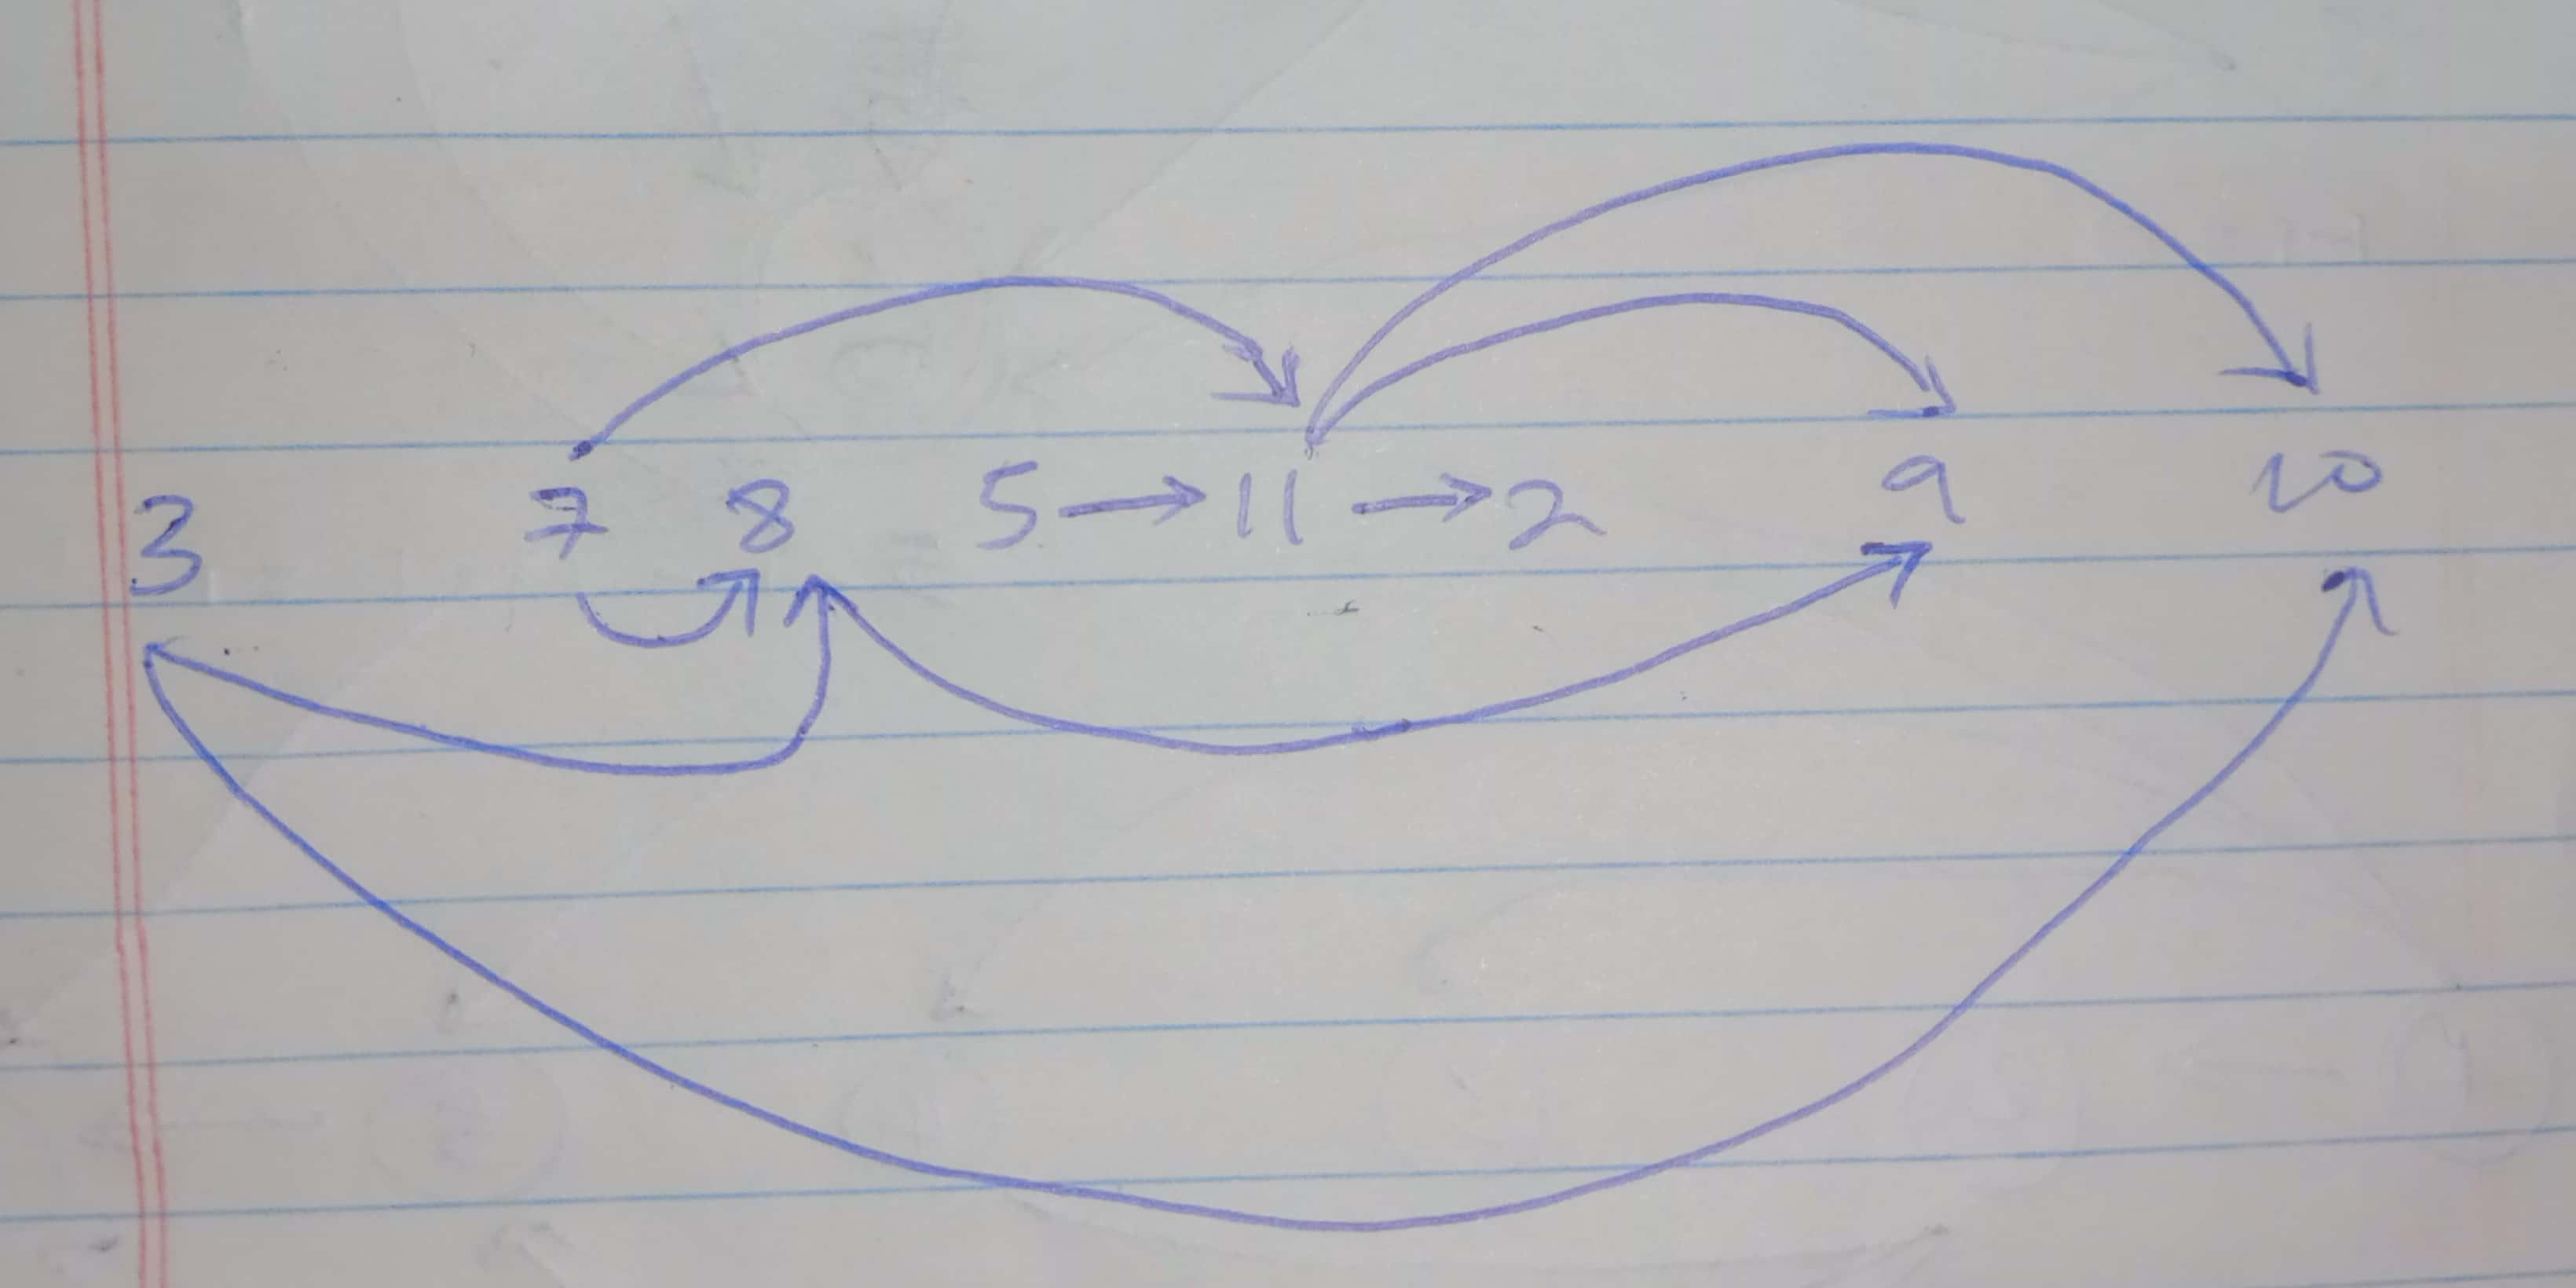
\includegraphics[width=0.8\textwidth]{toposort1.jpg}
\end{center}
\subsection*{b}
\begin{center}
    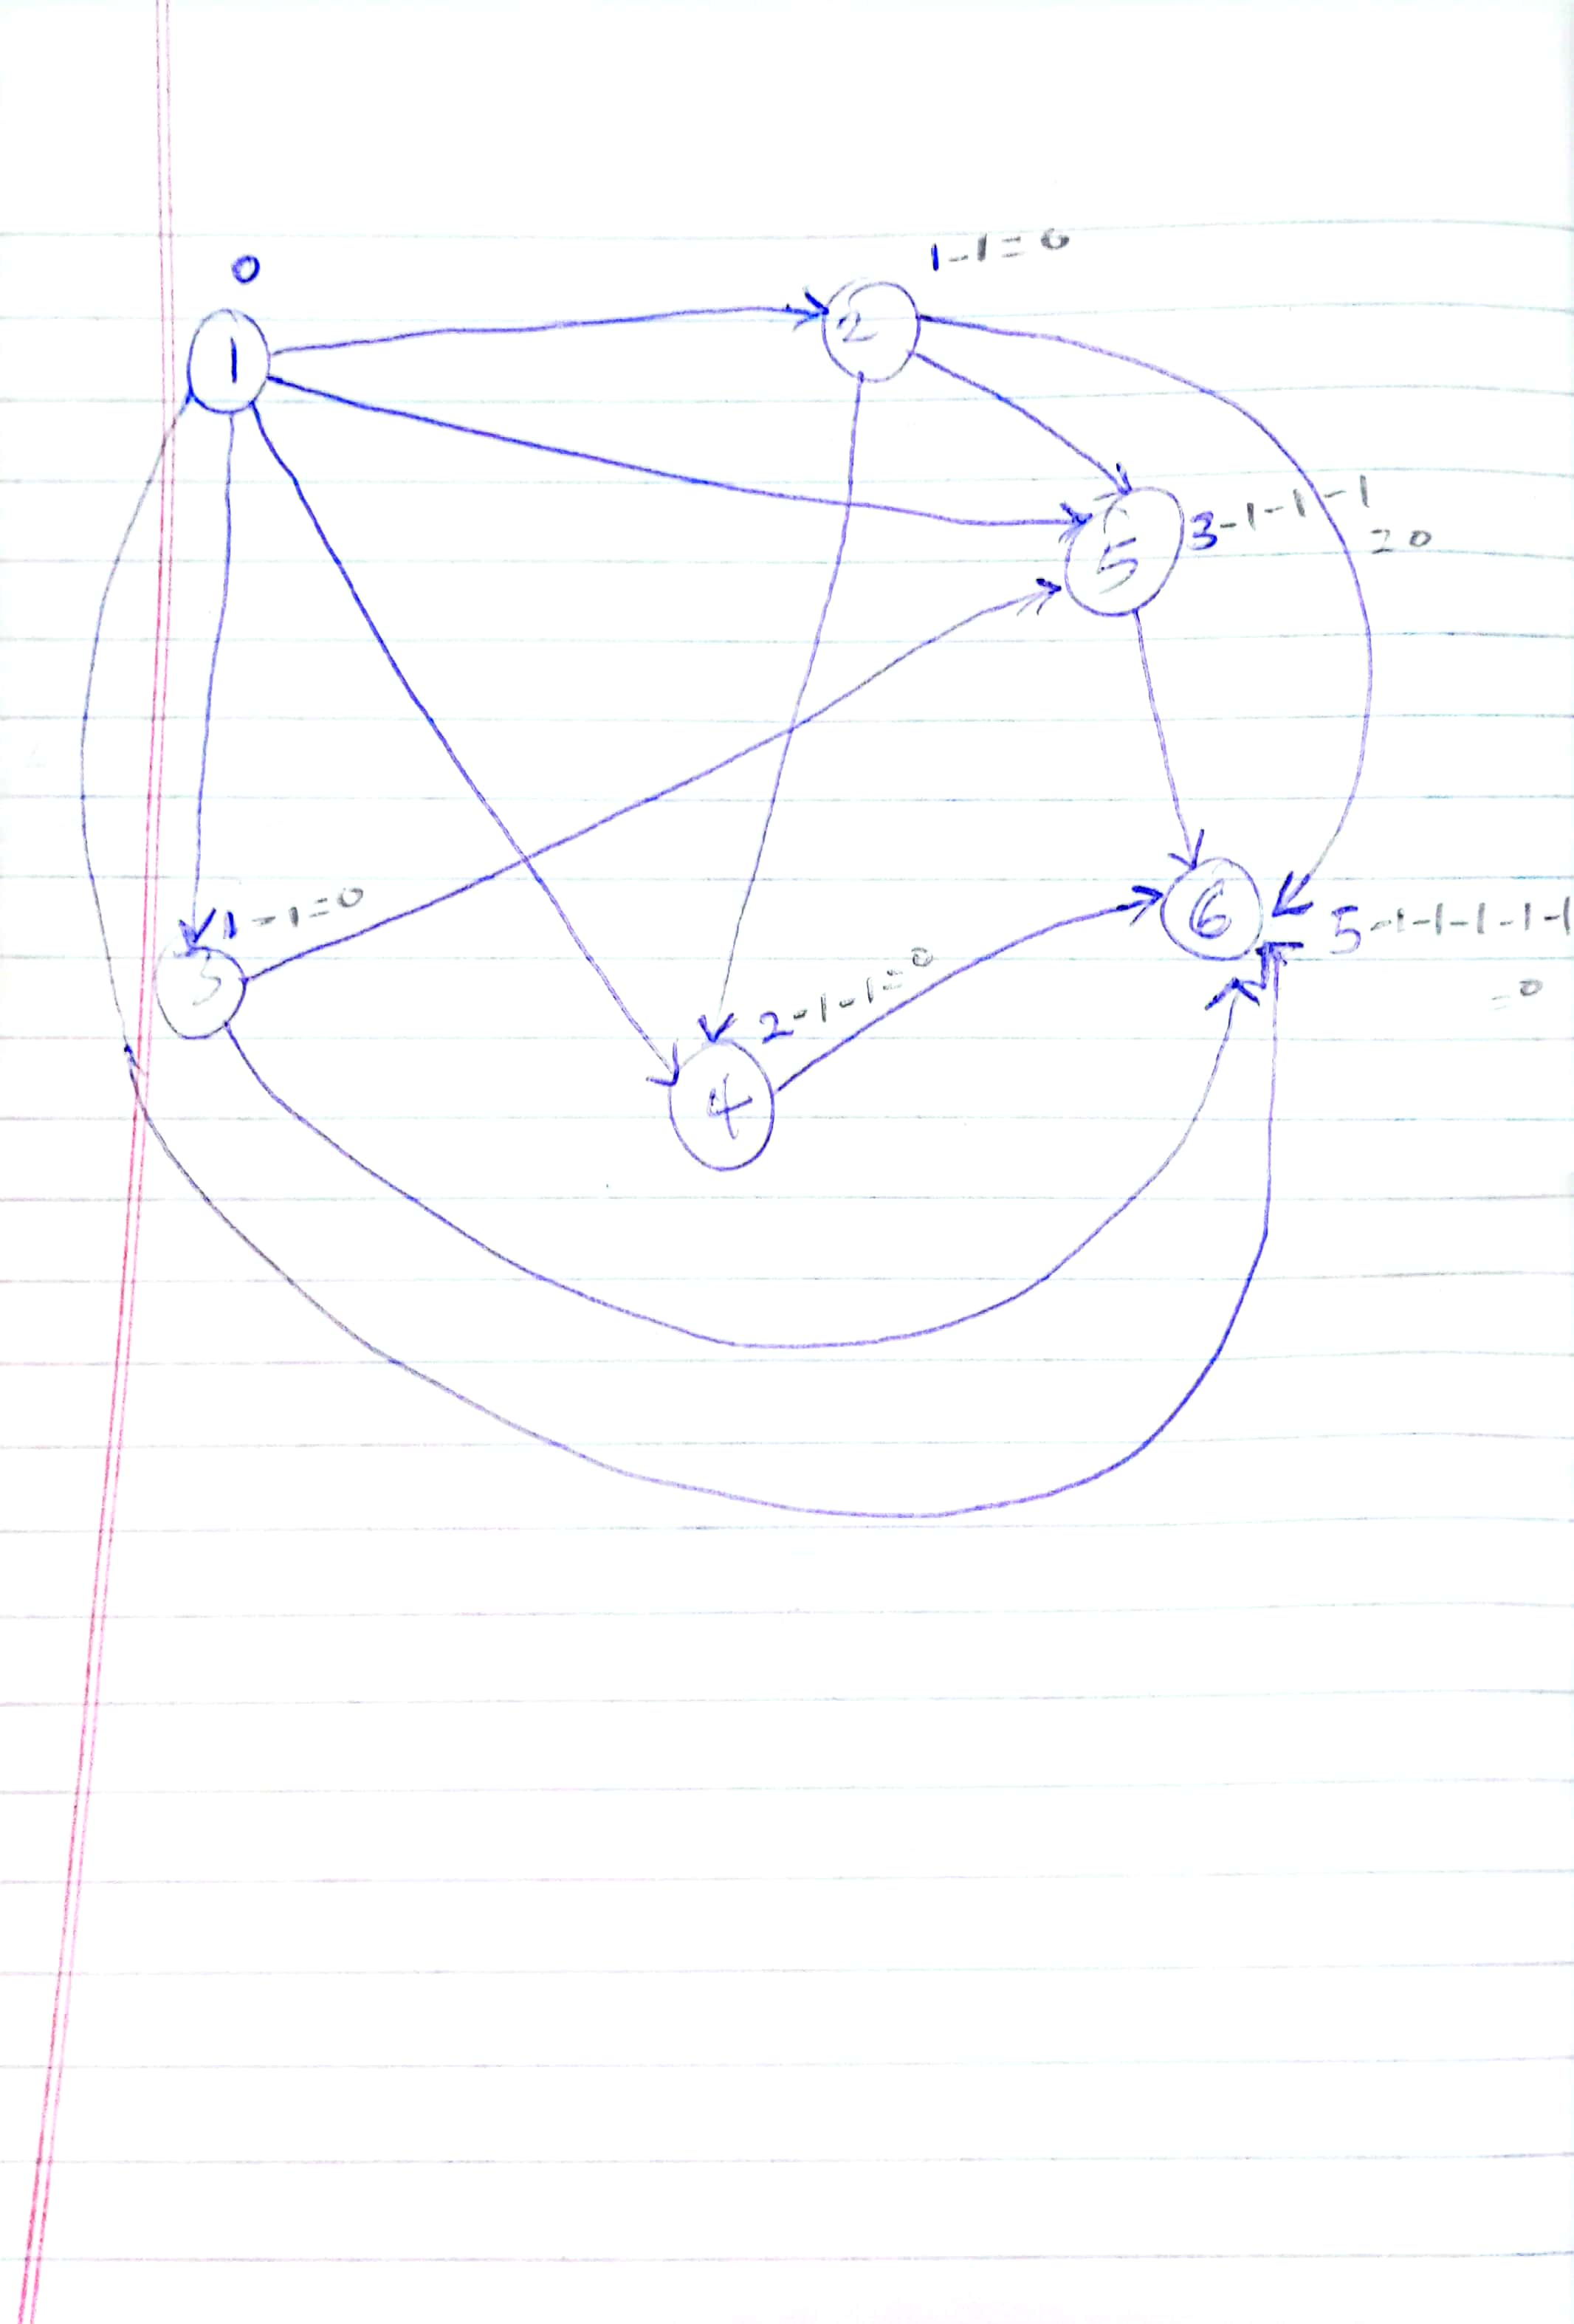
\includegraphics[width=0.8\textwidth]{toposort2.jpg}
    \newpage
    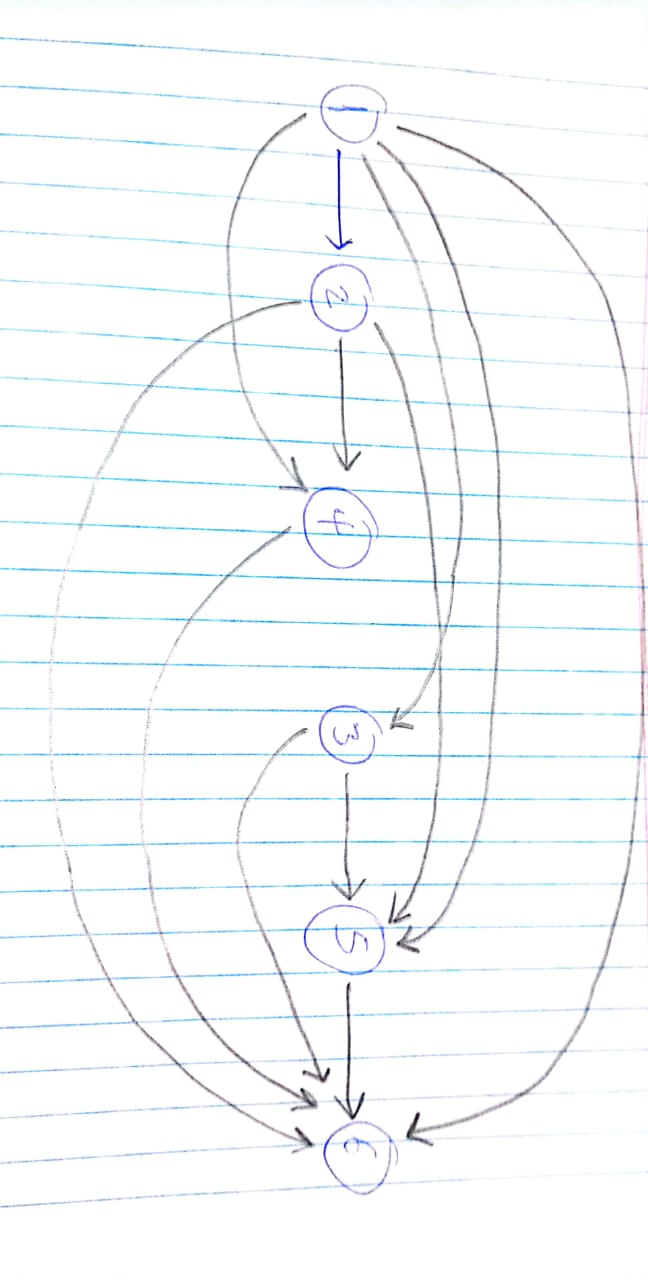
\includegraphics[width=0.8\textwidth]{toposort3.jpg}
\end{center}
\newpage
\section*{Question 5}
\subsection*{a}
\begin{itemize}
    \item Base Case (n = 1):
          For a magic square of order 1, it consists of a single cell with the value \( a_{11} \). The sum of any row, column, or diagonal is simply \( a_{11} \), which equals the only number present in the magic square. This sum is \( 1 \times (1^2 + 1)/2 = 1 \), satisfying the formula.

    \item Inductive Step:
          Assume that the sum is equal to \( n(n^2 + 1)/2 \) for a magic square of order \( n = k \), where \( k \geq 1 \).

    \item Consider a magic square of order \( n = k + 1 \). The sum must equal \( (k + 1)((k + 1)^2 + 1)/2 \)

          Consider the sum of the elements in the magic square of order \( n = k + 1 \). Each row, column, and diagonal in this magic square can be split into two parts: the elements from the magic square of order \( n = k \) and the additional elements in the last row and last column.

          By the induction hypothesis, the sum of the elements from the magic square of order \( n = k \) is \( k(k^2 + 1)/2 \).

          Consider the sum of the additional elements in the last row and last column. Since the numbers in these positions increase by \( k + 1 \) from the corresponding positions in the magic square of order \( n = k \), the sum of the elements in the last row and last column is \( (k + 1)(k + 1) = (k + 1)^2 \).

          Therefore, the total sum of the elements in the magic square of order \( n = k + 1 \) is \( k(k^2 + 1)/2 + (k + 1)^2 \).
\end{itemize}

Simplifying:

\[ \frac{k(k^2 + 1)}{2} + (k + 1)^2 = \frac{k^3 + k}{2} + (k^2 + 2k + 1) = \frac{k^3 + 3k^2 + 3k + 1}{2} \]

\[ = \frac{(k + 1)((k + 1)^2 + 1)}{2} \]

Thus, the sum for a magic square of order \( n = k + 1 \) is also equal to \( (k + 1)((k + 1)^2 + 1)/2 \).

By the principle of mathematical induction, the statement holds for all positive integers \( n \).

Therefore, if a magic square of order \( n \) exists, the sum must be equal to \( n(n^2 + 1)/2 \).

\subsection*{b}
\begin{verbatim}
    function GenerateMagicSquares(n):
        // Initialize an empty n x n matrix
        matrix = empty n x n matrix
    
        // Initialize a list to store all magic squares
        magicSquares = empty list
    
        // Call the generateSquares function to start generating magic squares
        generateSquares(matrix, 0, 0, magicSquares)
    
        // Return the list of all magic squares
        return magicSquares
    
    function generateSquares(matrix, row, col, magicSquares):
        // If the entire matrix is filled up
        if row == matrix.length and col == 0:
            // If the matrix is a magic square, add it to the list
            if isMagicSquare(matrix):
                magicSquares.add(copy of matrix)
            return
    
        // Calculate the next row and column
        nextRow, nextCol = (row, col + 1) if col + 1 < matrix.length else (row + 1, 0)
    
        // Try placing each number from 1 to n^2 in the current cell
        for num in 1 to n^2:
            // If the number is not already in the matrix
            if num not in matrix:
                // Place the number in the current cell
                matrix[row][col] = num
    
                // Recursively generate squares for the rest of the cells
                generateSquares(matrix, nextRow, nextCol, magicSquares)
    
                // Remove the number from the current cell (backtrack)
                matrix[row][col] = 0
    
    function isMagicSquare(matrix):
        magicConstant = sum of the first row of matrix
    
        for i in 0 to matrix.length - 1:
            if sum of row i != magicConstant or sum of column i != magicConstant:
                return false
    
        if sum of main diagonal != magicConstant or sum of secondary diagonal != magicConstant:
            return false
    
        // If all checks passed, the matrix is a magic square
        return true
    \end{verbatim}

\subsection*{c}
There are two popular methods for generating magic squares: the Siamese method for odd-order magic squares and the Square of Squares method for even-order magic squares. The Siamese method is a simple algorithm that starts by placing the number 1 at the middle of the top row and then fills in the numbers sequentially using specific rules. The Square of Squares method decomposes the square into four sub-squares and fills them with numbers sequentially to form a complete magic square.
\begin{verbatim}
    function GenerateMagicSquare(n):
        if n is odd:
            return SiameseMethod(n)
        else:
            return SquareOfSquaresMethod(n)
    
    function SiameseMethod(n):
        // Initialize an empty n x n matrix
        matrix = empty n x n matrix
        
        // Initialize the position for the first number
        row = 0
        col = n // 2
    
        // Fill in the numbers in the matrix using the Siamese method
        for num in 1 to n*n:
            matrix[row][col] = num
            // Calculate the next position based on the Siamese method rules
            nextRow = (row - 1 + n) % n
            nextCol = (col + 1) % n
            // If the next position is already filled, move down instead
            if matrix[nextRow][nextCol] != 0:
                nextRow = (row + 1) % n
                nextCol = col
            // Update the current position
            row = nextRow
            col = nextCol
    
        return matrix
    
    function SquareOfSquaresMethod(n):
        // Initialize an empty n x n matrix
        matrix = empty n x n matrix
    
        // Calculate the size of each sub-square
        subSize = n / 4
    
        // Generate sub-squares for each quadrant
        subMatrix1 = GenerateSubSquare(subSize)
        subMatrix2 = GenerateSubSquare(subSize)
        subMatrix3 = GenerateSubSquare(subSize)
        subMatrix4 = GenerateSubSquare(subSize)
    
        // Fill the main matrix with sub-squares
        for i in 0 to subSize-1:
            for j in 0 to subSize-1:
                matrix[i][j] = subMatrix1[i][j]
                matrix[i][j + subSize*2] = subMatrix2[i][j]
                matrix[i + subSize*2][j] = subMatrix3[i][j]
                matrix[i + subSize*2][j + subSize*2] = subMatrix4[i][j]
    
        return matrix
    
    function GenerateSubSquare(subSize):
        // Initialize an empty subSize x subSize matrix
        subMatrix = empty subSize x subSize matrix
        // Fill the sub-square with numbers sequentially
        num = 1
        for i in 0 to subSize-1:
            for j in 0 to subSize-1:
                subMatrix[i][j] = num
                num = num + 1
        return subMatrix
    \end{verbatim}

\subsubsection*{Explanation}
\begin{itemize}
    \item The GenerateMagicSquare function takes the order n of the magic square as input.
          If n is odd, it calls the SiameseMethod function to generate an odd-order magic square
          using the Siamese method. If n is even, it calls the SquareOfSquaresMethod function to
          generate an even-order magic square using the Square of Squares method.

    \item The SiameseMethod function generates an odd-order magic square using the Siamese method.
          It initializes an empty n x n matrix and starts by placing the number 1 at the middle of the
          top row. It then iteratively fills in the numbers in the matrix according to the Siamese
          method rules.

    \item The SquareOfSquaresMethod function generates an even-order magic square using the Square
          of Squares method. It decomposes the square into four sub-squares and fills them with numbers
          using the GenerateSubSquare function. It then arranges these sub-squares in the main matrix
          to form a complete magic square.

    \item The GenerateSubSquare function generates a sub-square of a specified size and fills it with
          consecutive numbers starting from 1. This function is used to generate each of the four
          sub-squares in the SquareOfSquaresMethod.
\end{itemize}

\subsection*{d}
\begin{itemize}
\item The exhaustive search algorithm was only able to generate magic squares of order 4 under 1 minute.
\item The non-exhaustive search algorithm (Siamese method for odd numbers, Square of Square method for even orders)
went up to order 876 under 1 minute.

\end{itemize}




\newpage



\end{document}
